\documentclass{beamer}
\usetheme{metropolis}
\usepackage{graphicx}
\usepackage{amsmath}
\usepackage{makecell}
\title{A History of Science in Latin America (INTD290): Unit 1.1}
\author{Jordan Hanson}
\institute{Whittier College Department of Physics and Astronomy}

\begin{document}
\maketitle

\section{Review}

\begin{frame}{Review}
\alert{Indigenous and Spanish Colonial Medicine}:
\begin{enumerate}
\item Indigenous medicine and science
\item Medieval medical theory
\begin{itemize}
\item The four humours
\item Hot/cold, wet/dry
\item Relation to elements, digestion
\end{itemize}
\item Comparisons of treatments: examples of indigenous science
\item Production of treatments
\begin{itemize}
\item Introduction from indigenous to colonial
\item Production and shipment to Europe
\end{itemize}
\end{enumerate}
\alert{Connections Activities}:
\begin{itemize}
\item The base-20 number system of the Maya
\item The Quipu of the Inca
\item Kepler's Laws
\end{itemize}
\end{frame}

\section{Outline}

\begin{frame}{Outline}
\textit{Comparitive medical treatments - chapter 1 content.} \\
\alert{Chapter 2 content}
\begin{enumerate}
\item Mining and agriculture in Nueva Espa\~{n}a
\item Construction of scientific communities
\item The formation of scientific literature and community, importation of scientific texts
\item Catholic religious orders in Latin America
\item Galileo, Kepler, and the Heliocentric system of the world
\end{enumerate}
\alert{Activities}
\begin{enumerate}
\item Timelines of discoveries and development
\item Geographical illustrations with Google Earth
\item Digital Storytelling on cosmic rays and the solar wind
\end{enumerate}
\end{frame}

\section{Comparitive Medical Treatments}

\begin{frame}{Comparitive Medical Treatments}
\small
The Nahua must have had intricate systems of medicinal practice:
\begin{table}
\centering
\begin{tabular}{| c | c | c | c |}
\hline
People & Disease & Cure & Notes \\ \hline \hline
European  & \textit{Dysentery} & \makecell{Manure with wine \\ vinegar \\ ground pig feet with wine \\ dog urine with wine} & \makecell{Acidic things \\ change microfauna} \\ \hline
\end{tabular}
\begin{tabular}{| c | c | c | c |}
\hline
People & Disease & Cure & Notes \\ \hline \hline
Nahua & \textit{Diarrhea} & \makecell{tzipipatli boiled in water \\ atole with chia, tortilla \\ xalxocotl fruit, leaves} & \makecell{herbal things \\ breastmilk to baby} \\ \hline
\end{tabular}
\end{table}
\end{frame}

\begin{frame}{Comparitive Medical Treatments}
\small
The Nahua must have had intricate systems of medicinal practice:
\begin{table}
\centering
\begin{tabular}{| c | c | c | c |}
\hline
People & Disease & Cure & Notes \\ \hline \hline
European  & \textit{Broken ribs} & \makecell{Dry ground goat manure \\ baked with wine \\ plastered to ribs} & \makecell{No idea, honestly} \\ \hline
\end{tabular}
\begin{tabular}{| c | c | c | c |}
\hline
People & Disease & Cure & Notes \\ \hline \hline
Nahua & \textit{Broken bone} & \makecell{Push then stretched \\ zacacili poultice with splint \\ Cut with obsidian knife \\ Apply iztaczazalic \\ + tememetatl to cut} & \makecell{Bone setting, \\ \textit{\makecell{Ipomoea flowers \\ are entheogens}}} \\ \hline
\end{tabular}
\end{table}
Notice that the Europeans had metal knives, but did not have the drugs to ease pain and swelling. \textit{Tesoro de medicinas - Gregorio L\'{o}pez.}
\end{frame}

\begin{frame}{Comparative Medical Treatments}
\begin{enumerate}
\item Father Bernardino de Sahag\'{u}n compiled dictations from Mexican doctors who dictated it from Nahuatl.
\item Many indigenous manuscripts were censored by the Catholic Church
\begin{itemize}
\item Ipomoea flowers were also used in pagan rituals
\item One effect is the ego dissolution, the feeling that ``you'' are gone
\item Another example is \textit{salvia divinorum} - Herba de Maria
\end{itemize}
\item Why is a Catholic priest passing on this knowledge?
\item Similar process for the quipu
\end{enumerate}
\end{frame}

\section{Side Story: Roald Amundsen and the Netsilik}

\begin{frame}{Side Story - Comparitive Medicine and Exploration Done Right}
\small
\textbf{Professor: launch Google Earth}
\begin{enumerate}
\item The Northwest Passage
\item Scurvy and mistaken cause of tainted food
\begin{itemize}
\item Artic cloudberry - Vikings
\item But those aren't in Canada ... not in winter.
\end{itemize}
\item Physics and sleds
\end{enumerate}
\url{https://www.canadiangeographic.ca/article/}
\url{lessons-northwest-passage-roald-amundsens-experiences}
\url{-canadian-arctic}
\end{frame}

\section{Founding of Technical Colleges in Nueva Espa\~{n}a, Nueva Granada, y Per\'{u}}

\begin{frame}{Founding of Technical Colleges}
\begin{figure}
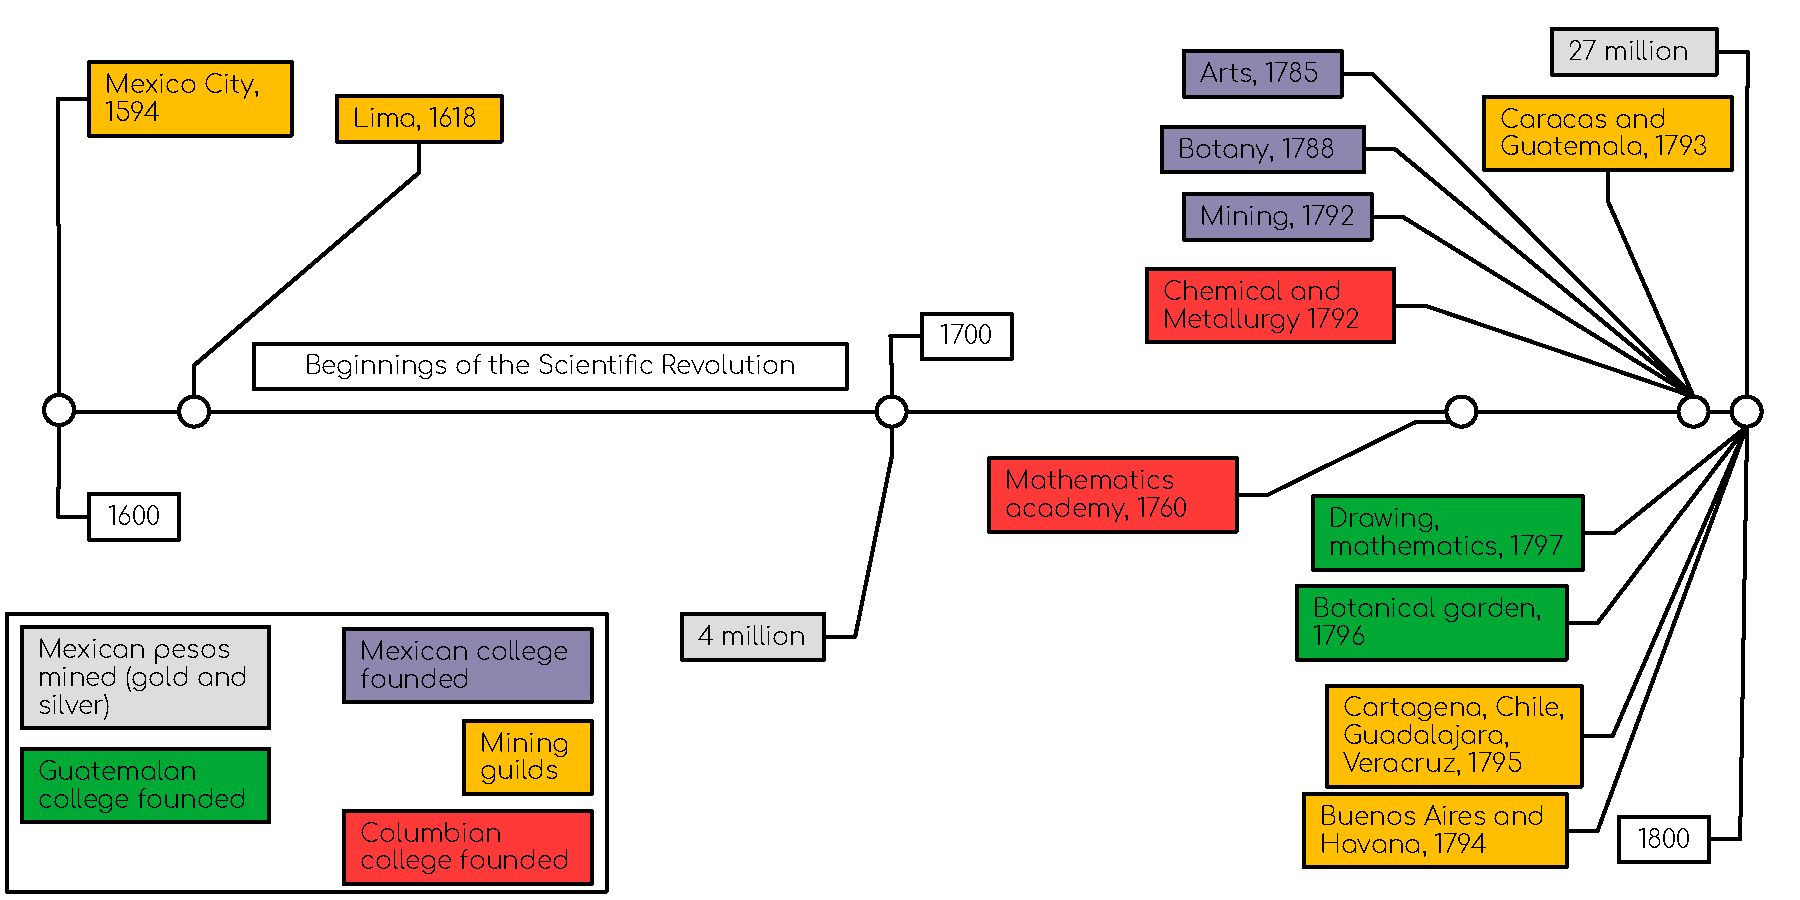
\includegraphics[width=10cm]{figures/Timeline.pdf}
\caption{\label{fig:timeline} A timeline of mining, founding of colleges, and production across several viceroyalties.}
\end{figure}
\end{frame}

\section{Activity: The Pierre Auger Observatory}

\begin{frame}{PAO in Google Earth}
\begin{enumerate}
\item What is a cosmic ray?
\item Review Cherenkov radiation
\item Two techniques for observing them
\item Google Earth
\end{enumerate}
\end{frame}

\begin{frame}{PAO in Google Earth}
\begin{figure}
\centering
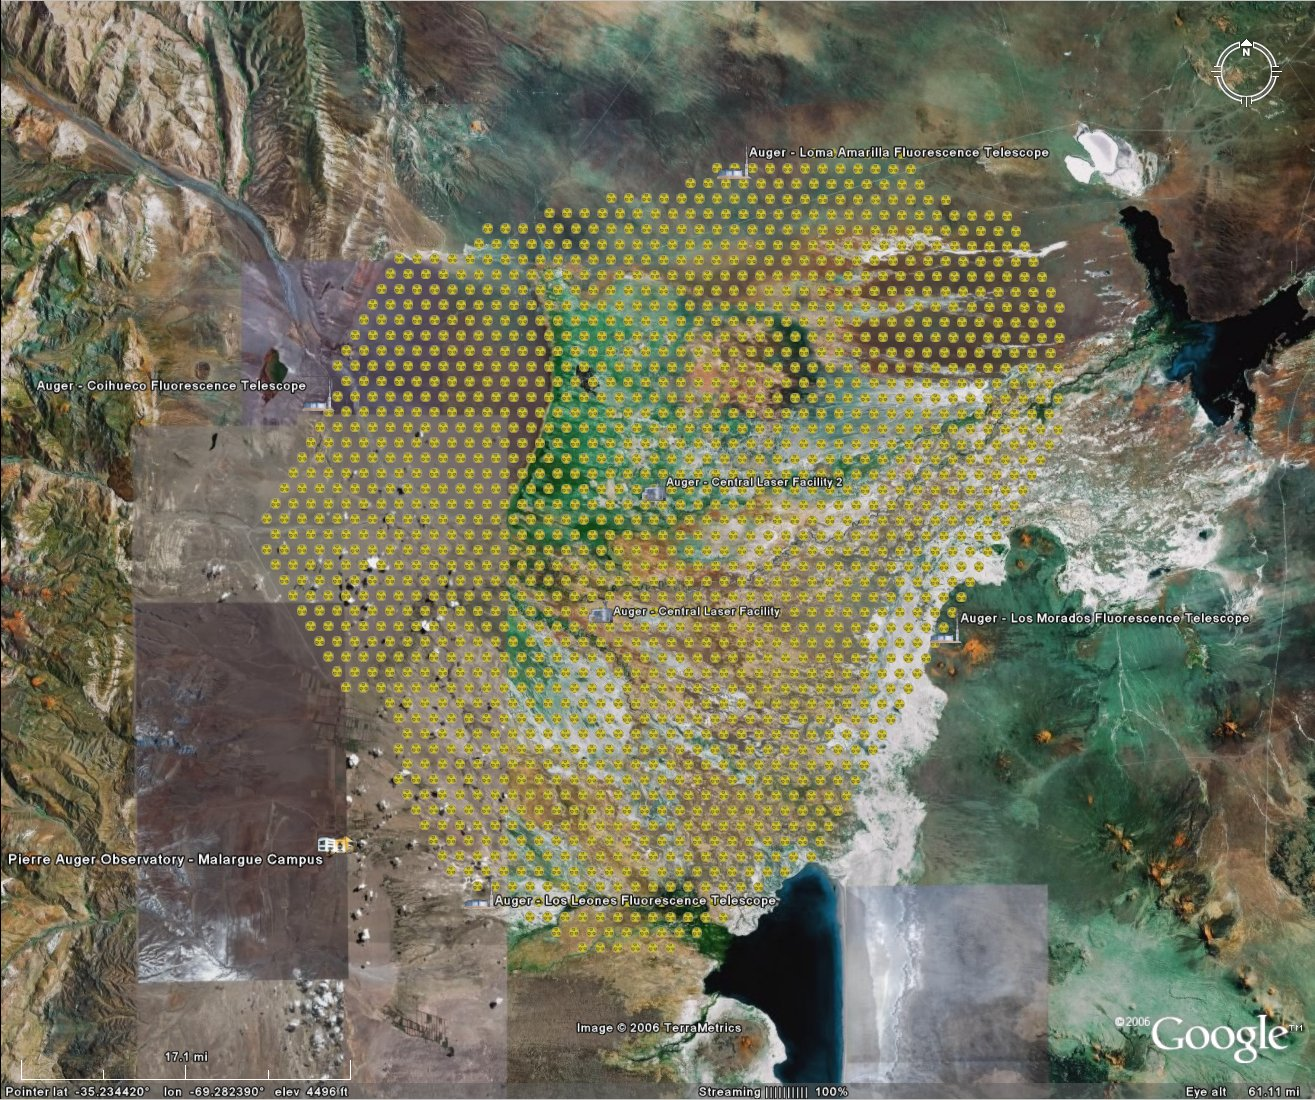
\includegraphics[width=8cm]{figures/Auger.jpg}
\caption{\label{fig:aug} The entire PAO detector layout.}
\end{figure}
\end{frame}

\end{document}